%!TEX TS-program = xelatex
%!TEX encoding = UTF-8 Unicode
% Awesome CV LaTeX Template for CV/Resume
%
% This template has been downloaded from:
% https://github.com/posquit0/Awesome-CV
%
% Author:
% Claud D. Park <posquit0.bj@gmail.com>
% http://www.posquit0.com
%
%
% Adapted to be an Rmarkdown template by Mitchell O'Hara-Wild
% 23 November 2018
%
% Template license:
% CC BY-SA 4.0 (https://creativecommons.org/licenses/by-sa/4.0/)
%
%-------------------------------------------------------------------------------
% CONFIGURATIONS
%-------------------------------------------------------------------------------
% A4 paper size by default, use 'letterpaper' for US letter
\documentclass[11pt,a4paper,]{awesome-cv}

% Configure page margins with geometry
\usepackage{geometry}
\geometry{left=1.4cm, top=.8cm, right=1.4cm, bottom=1.8cm, footskip=.5cm}


% Specify the location of the included fonts
\fontdir[fonts/]

% Color for highlights
% Awesome Colors: awesome-emerald, awesome-skyblue, awesome-red, awesome-pink, awesome-orange
%                 awesome-nephritis, awesome-concrete, awesome-darknight

\definecolor{awesome}{HTML}{207373}

% Colors for text
% Uncomment if you would like to specify your own color
% \definecolor{darktext}{HTML}{414141}
% \definecolor{text}{HTML}{333333}
% \definecolor{graytext}{HTML}{5D5D5D}
% \definecolor{lighttext}{HTML}{999999}

% Set false if you don't want to highlight section with awesome color
\setbool{acvSectionColorHighlight}{true}

% If you would like to change the social information separator from a pipe (|) to something else
\renewcommand{\acvHeaderSocialSep}{\quad\textbar\quad}

\def\endfirstpage{\newpage}

%-------------------------------------------------------------------------------
%	PERSONAL INFORMATION
%	Comment any of the lines below if they are not required
%-------------------------------------------------------------------------------
% Available options: circle|rectangle,edge/noedge,left/right

\photo{../images/JDL.jpg}
\name{Juan David}{Leongómez}

\position{Associate Professor}
\address{Faculty of Psychology, Universidad El Bosque}

\mobile{(+57) 601-6489000 Ext. 1901}
\email{\href{mailto:jleongomez@unbosque.edu.co}{\nolinkurl{jleongomez@unbosque.edu.co}}}
\homepage{jdleongomez.info}
\orcid{0000-0002-0092-6298}

% \gitlab{gitlab-id}
% \stackoverflow{SO-id}{SO-name}
% \skype{skype-id}
% \reddit{reddit-id}

\quote{I am a researcher mainly interested in human behaviour, as well
as quantitative methods and reproducible science.}

\usepackage{booktabs}

\providecommand{\tightlist}{%
	\setlength{\itemsep}{0pt}\setlength{\parskip}{0pt}}

%------------------------------------------------------------------------------



% Pandoc CSL macros
\newlength{\cslhangindent}
\setlength{\cslhangindent}{1.5em}
\newlength{\csllabelwidth}
\setlength{\csllabelwidth}{2em}
\newenvironment{CSLReferences}[3] % #1 hanging-ident, #2 entry spacing
 {% don't indent paragraphs
  \setlength{\parindent}{0pt}
  % turn on hanging indent if param 1 is 1
  \ifodd #1 \everypar{\setlength{\hangindent}{\cslhangindent}}\ignorespaces\fi
  % set entry spacing
  \ifnum #2 > 0
  \setlength{\parskip}{#2\baselineskip}
  \fi
 }%
 {}
\usepackage{calc}
\newcommand{\CSLBlock}[1]{#1\hfill\break}
\newcommand{\CSLLeftMargin}[1]{\parbox[t]{\csllabelwidth}{\honortitlestyle{#1}}}
\newcommand{\CSLRightInline}[1]{\parbox[t]{\linewidth - \csllabelwidth}{\honordatestyle{#1}}}
\newcommand{\CSLIndent}[1]{\hspace{\cslhangindent}#1}

\begin{document}

% Print the header with above personal informations
% Give optional argument to change alignment(C: center, L: left, R: right)
\makecvheader

% Print the footer with 3 arguments(<left>, <center>, <right>)
% Leave any of these blank if they are not needed
% 2019-02-14 Chris Umphlett - add flexibility to the document name in footer, rather than have it be static Curriculum Vitae
\makecvfooter
  {15 February, 2023}
    {Juan David Leongómez~~~·~~~Academic Curriculum Vitae}
  {\thepage}


%-------------------------------------------------------------------------------
%	CV/RESUME CONTENT
%	Each section is imported separately, open each file in turn to modify content
%------------------------------------------------------------------------------



\hypertarget{about-me}{%
\section{About me}\label{about-me}}

\begin{minipage}[c]{0.85\linewidth}
I am an Associate Professor and Researcher at \href{https://jdleongomez.info/en/team/}{\textit{\textbf{EvoCo}: Human Behaviour and Evolution Lab}}, and leader of the \href{https://investigaciones.unbosque.edu.co/codec}{\textit{\textbf{CODEC}: Cognitive and Behavioural Sciences}} research group (classification \href{https://scienti.minciencias.gov.co/gruplac/jsp/visualiza/visualizagr.jsp?nro=00000000001446}{\textbf{A1}}), \href{https://www.uelbosque.edu.co/psicologia}{Faculty of Psychology}, at \href{https://www.uelbosque.edu.co/}{Universidad El Bosque} in Bogota, Colombia. My research interests mostly lie in mate choice, human vocal communication, and musicality, as well as bioacoustics, psychoacoustics, and hormonal effects on human behaviour. I published among the first articles showing within-individual changes in voice pitch in response to the social status of the listener, and have demonstrated strong effects of voice modulation on listeners in courtship contexts. I am very passionate about quantitative methods and \textbf{R} programming, as a tool to promote reproducibility and open science. Consequently, I am a \href{https://rr.peercommunityin.org/about/recommenders}{recommender} (editor) for \href{https://rr.peercommunityin.org/}{PCI Registered Reports}.
\end{minipage} \begin{minipage}[c]{0.15\linewidth}
\begin{flushright} 
\hfill \href{https://jdleongomez.info/en/team/}{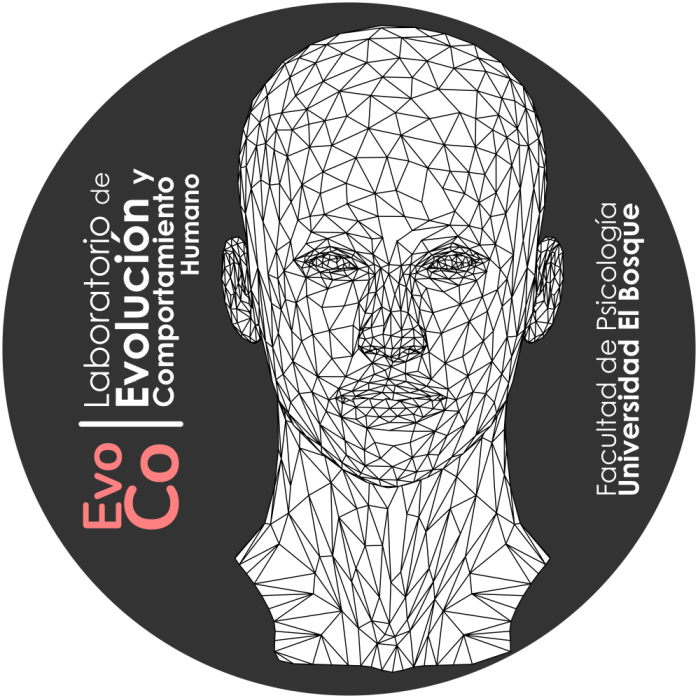
\includegraphics[width=2.3cm, height=2.3cm]{Logo_EvoCo.png}} \newline \href{https://investigaciones.unbosque.edu.co/codec}{
\includegraphics[width=2.3cm, height=2.3cm]{Logo_CODEC.png}}
\end{flushright}
\end{minipage}

\hypertarget{skills}{%
\section{Skills}\label{skills}}

\begin{cvskills}
  \cvskill
    {Programming}
    {\href{https://www.r-project.org/}{\textbf{R}} (advanced: all data wrangling, analysis, plots and tables -and even this CV- made in R)}

  \cvskill
    {Reproducible Reports}
    {Markdown/\href{https://rmarkdown.rstudio.com/}{R Markdown} (including {\fontfamily{cmr}\selectfont\LaTeX} and HTML\faHtml5). Version control: \href{https://git-scm.com/}{Git} \faGit* and \href{https://github.com/JDLeongomez}{GitHub} \faGithub}

  \cvskill
    {Quantitative Research}
    {General and generalised models, linear mixed-effects models, multi-model inference, machine learning}

  \cvskill
    {Software}
    {\href{https://posit.co/products/open-source/rstudio/}{RStudio}, \href{https://code.visualstudio.com/}{Visual Studio Code}, \href{https://www.fon.hum.uva.nl/praat/}{Praat}, \href{https://www.audacityteam.org/}{Audacity}, \href{https://inkscape.org/}{InkScape}, \href{https://www.zotero.org/}{Zotero}}

  \cvskill
    {Languages}
    {English/Spanish (native)}
\end{cvskills}

\hypertarget{research}{%
\section{Research}\label{research}}

\begin{cvskills}
  \cvskill
    {Research Areas}
    {\textbf{Human voice • Vocal modulation • Mate choice • Human behaviour}}

  \cvskill
    {Primary Research Methods}
    {Experimental designs • Acoustic analysis • Geometric morphometrics • Stimuli rating}
\end{cvskills}

\hypertarget{education}{%
\section{Education}\label{education}}

\begin{cventries}
    \cventry{PhD - Psychology}{\href{https://www.stir.ac.uk/}{University of Stirling}}{Stirling, UK}{2014}{\begin{cvitems}
\item Dissertation \href{https://dspace.stir.ac.uk/handle/1893/21102}{\textbf{\textit{Contextual musicality: vocal modulation and its perception in human social interaction}}}
\item Supervisors: \href{https://www.scraigroberts.com/}{Prof. S. Craig Roberts} and \href{https://scholar.google.com/citations?user=iDDoxVsAAAAJ}{Prof. Anthony C. Little}
\item Committee members: \href{https://scholar.google.co.uk/citations?user=wxh9svQAAAAJ}{Prof. Phyllis C. Lee} (dissertation chair) and \href{https://scholar.google.com/citations?user=Qo23OGoAAAAJ}{Prof. Stuart Semple}
\end{cvitems}}
    \cventry{MSc in Evolutionary Psychology}{\href{https://www.liverpool.ac.uk/}{University of Liverpool}}{Liverpool, UK}{2009}{\begin{cvitems}
\item Supervisor: \href{https://www.scraigroberts.com/}{Prof. S. Craig Roberts}
\item Best overall performance in the MSc
\end{cvitems}}
    \cventry{BA in Music Pedagogy}{\href{https://www.upn.edu.co/}{Universidad Pedagógica Nacional}}{Bogota, Colombia}{2006}{\begin{cvitems}
\item GPA: 4.28/5.00
\item Research project: 4.90/5.00
\end{cvitems}}
\end{cventries}

\hypertarget{relevant-further-education}{%
\section{Relevant further education}\label{relevant-further-education}}

\begin{cventries}
    \cventry{Practical Machine Learning}{Johns Hopkins University}{Coursera (MOOC platform)}{2021}{\begin{cvitems}
\item GPA: 97/100 (see \href{https://www.coursera.org/account/accomplishments/verify/DC7ULMJ3CZWM}{certificate})
\end{cvitems}}
    \cventry{Statistical Programming in R and Linear Mixed Models}{University of Dundee}{Dundee, UK}{2012}{}\vspace{-4.0mm}
\end{cventries}

\hypertarget{working-experience}{%
\section{Working Experience}\label{working-experience}}

\begin{cventries}
    \cventry{Associate Professor}{\href{https://www.unbosque.edu.co/}{Universidad El Bosque}}{Bogota, Colombia}{Apr. 2019 - Present}{\begin{cvitems}
\item Researcher at \href{https://jdleongomez.info/es/team/}{\textit{\textbf{EvoCo}: Human Behaviour and Evolution Lab}}
\item Leader of the \href{https://investigaciones.unbosque.edu.co/codec}{\textit{\textbf{CODEC}: Cognitive and Behavioural Sciences}} research group (since 2016)
\item \href{https://asesores-psic.netlify.app/}{Methodological and statistical advisor} for postgraduate and faculty research projects
\item Supervision of a variety of undergraduate research projects associated with psychology and biology
\item Member of the Research Committee
\item Member of the Advisory Committee on Research Ethics
\end{cvitems}}
    \cventry{Assistant Professor}{\href{https://www.unbosque.edu.co/}{Universidad El Bosque}}{Bogota, Colombia}{Jan. 2015 - Apr. 2019}{\begin{cvitems}
\item Researcher at \href{https://jdleongomez.info/es/team/}{\textit{\textbf{EvoCo}: Human Behaviour and Evolution Lab}}
\item Leader of the \href{https://investigaciones.unbosque.edu.co/codec}{\textit{\textbf{CODEC}: Cognitive and Behavioural Sciences}} research group (since 2016)
\item \href{https://asesores-psic.netlify.app/}{Methodological and statistical advisor} for postgraduate and faculty research projects
\item Organiser of the Nerd Café weekly conference series of the Faculty of Psychology (2016-2017)
\item Supervision of a variety of undergraduate research projects associated with psychology and biology
\item Postdoctoral stay (2018-2019)
\item Co-supervision of Doctoral Students:  \href{https://www.researchgate.net/profile/Milena-Vasquez-Amezquita}{Milena Vásquez-Amézquita} (PhD in Neuroscience, University of Valencia, Spain – 2015-2018)
\item Co-supervision of Doctoral Students:  Francisco Javier Flores (Professional Doctorate in Counselling Psychology, University of East London, UK – 2016‑2018)
\end{cvitems}}
    \cventry{Cathedratic Professor}{\href{https://www.unisabana.edu.co/}{Universidad de La Sabana}}{Chia, Colombia}{Jan. 2015 - Dec. 2016}{\begin{cvitems}
\item Teaching and supervision of research projects
\end{cvitems}}
    \cventry{Teaching Assistant}{\href{https://www.stir.ac.uk/}{University of Stirling}}{Stirling, UK}{2011 - 2014}{\begin{cvitems}
\item Supervision of an MSc research project (Evolutionary Psychology MSc)
\item Marking and statistical advice to MSc students
\end{cvitems}}
    \cventry{Auxiliar Professor}{\href{https://www.upn.edu.co/}{Universidad Pedagógica Nacional}}{Bogota, Colombia}{2010}{\begin{cvitems}
\item Member of the Research Committee
\item Supervision of research projects
\end{cvitems}}
\end{cventries}

\hypertarget{teaching-experience}{%
\section{Teaching Experience}\label{teaching-experience}}

\begin{cventries}
    \cventry{Associate Professor}{\href{https://www.unbosque.edu.co/}{Universidad El Bosque}}{Bogota, Colombia}{2019}{\begin{cvitems}
\item Quantitative Methods II (Psychology MSc) (2019)
\end{cvitems}}
    \cventry{Assistant Professor}{\href{https://www.unbosque.edu.co/}{Universidad El Bosque}}{Bogota, Colombia}{2015 - 2018}{\begin{cvitems}
\item Quantitative Methods II (Psychology MSc) (2017-2018)
\item Research Degree Project (2018)
\item Quantitative Methods I (Psychology MSc) (2017)
\item Sources and Documentation Styles in Psychology (2015)
\end{cvitems}}
    \cventry{Cathedratic Professor}{\href{https://www.unisabana.edu.co/}{Universidad de La Sabana}}{Chia, Colombia}{2015 - 2016}{\begin{cvitems}
\item Evolution and Development of Vocal Communication: Songs, Fashion, and Language (2016)
\item Inferential Statistics (2015 - 2016)
\item Descriptive Statistics (2015 - 2016)
\end{cvitems}}
    \cventry{Teaching Assistant}{\href{https://www.stir.ac.uk/}{University of Stirling}}{Stirling, UK}{2012 - 2014}{\begin{cvitems}
\item Animal Behaviour (lecture on vocal communication) (2012)
\item Quantitative Methods (Psychology MSc – several lectures, practical supervision, one-on-one teaching) (2012-2014)
\item Cognition Module (leading research projects in psychoacoustics) (2012-2014)
\end{cvitems}}
    \cventry{Auxiliar Professor}{\href{https://www.upn.edu.co/}{Universidad Pedagógica Nacional}}{Bogota, Colombia}{2010}{\begin{cvitems}
\item Research Project I (2010)
\item Research Lab II (2010)
\end{cvitems}}
\end{cventries}

\hypertarget{scholarships-awards-and-honors}{%
\section{Scholarships, Awards and
Honors}\label{scholarships-awards-and-honors}}

\begin{cventries}
    \cventry{IX Excellence Awards}{\href{https://www.unbosque.edu.co/}{Universidad El Bosque}}{Bogota, Colombia}{Dic. 2022}{\begin{cvitems}
\item COP\$10.000.000
\end{cvitems}}
    \cventry{Economics Prize}{\href{https://improbable.com/ig/about-the-ig-nobel-prizes/}{Ig Nobel Prize}}{Cambridge, MA, USA.}{Sep. 2020}{\begin{cvitems}
\item For ‘trying to quantify the relationship between different countries’ national income inequality and the average amount of mouth-to-mouth kissing’  (\href{https://doi.org/10.1038/s41598-019-43267-7}{Watkins, et al., 2019})
\end{cvitems}}
    \cventry{VIII Excellence Awards}{\href{https://www.unbosque.edu.co/}{Universidad El Bosque}}{Bogota, Colombia}{Dic. 2019}{\begin{cvitems}
\item COP\$7.000.000
\end{cvitems}}
    \cventry{VII Excellence Awards}{\href{https://www.unbosque.edu.co/}{Universidad El Bosque}}{Bogota, Colombia}{Dic. 2018}{\begin{cvitems}
\item COP\$5.000.000
\end{cvitems}}
    \cventry{VI Excellence Awards}{\href{https://www.unbosque.edu.co/}{Universidad El Bosque}}{Bogota, Colombia}{Dic. 2017}{\begin{cvitems}
\item COP\$5.000.000
\end{cvitems}}
    \cventry{Grindley Grants}{\href{https://eps.ac.uk/}{Experimental Psychology Society}}{Canterbury, UK}{Sep. 2014}{}\vspace{-4.0mm}
    \cventry{Francisco José de Caldas Scholarship for Doctoral Studies}{\href{https://minciencias.gov.co/}{Minciencias}}{Bogota, Colombia}{Oct. 2010 - Oct. 2014}{}\vspace{-4.0mm}
    \cventry{Annual Prize in Evolutionary Psychology}{\href{https://www.liverpool.ac.uk/life-sciences/}{School of Life Sciences} – University of Liverpool}{Liverpool, UK}{Oct. 2009}{\begin{cvitems}
\item Best overall performance in the MSc
\end{cvitems}}
    \cventry{University of Liverpool International Scholarship}{\href{https://www.liverpool.ac.uk/}{University of Liverpool}}{Liverpool, UK}{Sep. 2008 - Sep. 2009}{}\vspace{-4.0mm}
    \cventry{Scholarship-Loan Programme}{\href{https://www.colfuturo.org/}{Colfuturo}}{Bogota, Colombia}{Sep. 2008 - Sep. 2009}{}\vspace{-4.0mm}
\end{cventries}

\hypertarget{grants}{%
\section{Grants}\label{grants}}

\begin{cventries}
    \cventry{\href{https://minciencias.gov.co/convocatorias/investigacion/convocatoria-programa-estancias-postdoctorales-beneficiarios-colciencias}{Postdoctoral Research Stays - Colciencias beneficiaries 2017}}{\href{https://minciencias.gov.co/}{Minciencias}}{Bogota, Colombia}{Jan. 2018 - Jan. 2019}{\begin{cvitems}
\item Project: Perceptible signals of physical and mental health in faces, voices and body odors, and their relationship with hormonal levels
\item COP\$84.000.000
\end{cvitems}}
    \cventry{IX \href{https://www.unbosque.edu.co/investigaciones/convocatorias-investigacion}{Internal Call for Financing Research and Technological Innovation Projects El Bosque University}, 2017}{\href{https://www.unbosque.edu.co/}{Universidad El Bosque}}{Bogota, Colombia}{Jan. 2018 - Dec. 2021}{\begin{cvitems}
\item Project: Perceptible signals of physical and mental health in faces, voices and body odors, and their relationship with hormonal levels
\item COP\$136.586.537
\end{cvitems}}
    \cventry{VIII \href{https://www.unbosque.edu.co/investigaciones/convocatorias-investigacion}{Internal Call for Financing Research and Technological Innovation Projects El Bosque University}, 2016}{\href{https://www.unbosque.edu.co/}{Universidad El Bosque}}{Bogota, Colombia}{Jan. 2017 - Dec. 2020}{\begin{cvitems}
\item Project: Effects of evolutionary relevant static signals (sex, dominance, and attractiveness) on the cortical processing of human faces
\item COP\$80.000.000
\end{cvitems}}
    \cventry{VII \href{https://www.unbosque.edu.co/investigaciones/convocatorias-investigacion}{Internal Call for Financing Research and Technological Innovation Projects El Bosque University}, 2015}{\href{https://www.unbosque.edu.co/}{Universidad El Bosque}}{Bogota, Colombia}{Jan. 2016 - Dec. 2019}{\begin{cvitems}
\item Project: Effects of hormone levels, masculinity and femininity, on pitch discrimination in men and women
\item COP\$13.000.000
\end{cvitems}}
\end{cventries}

\hypertarget{publications}{%
\section{Publications}\label{publications}}

\hypertarget{section}{%
\subsection{\texorpdfstring{\textbf{Published Journal Articles and Works}}{}}\label{section}}

\begingroup
\setlength{\parindent}{-0.5in}
\setlength{\leftskip}{0.5in}

Vásquez-Amézquita, M., \textbf{Leongómez, J. D.}, Salvador, A., \& Seto,
M. C. (in press). What can the eyes tell us about atypical sexual
preferences as a function of sex and age? Linking eye movements with
child-related chronophilias. \emph{Forensic Sciences Research}.
\url{https://jdleongomez.info/en/files/eye-tracking_review.pdf}

\textbf{Leongómez, J. D.}, Havlíček, J., \& Roberts, S. C. (2022).
Musicality in Human Vocal Communication: An Evolutionary Perspective.
\emph{Philosophical Transactions of the Royal Society B: Biological
Sciences, 377}, 20200391. \url{https://doi.org/10.1098/rstb.2020.0391}

Santamaría-García, H., Burgaleta, M., Legaz, A., Flichtentrei, D.,
Cordoba-Delgado, M., Molina, J., Linares, J., Montealegre, J.,
Castelblanco Toro, S., Schulte, M., Paramo, J., Mondragón, I.,
\textbf{Leongómez, J. D.}, Salamone, P., González‑Pacheco, J., Baez, S.,
\& Ibañez, A.(2022). The price of prosociality in pandemic times.
\emph{Humanities and Social Sciences Communications, 9}, 15.
\url{https://doi.org/10.1057/s41599-021-01022-2}

Vásquez-Amézquita, M., Salvador, A., \& \textbf{Leongómez, J. D.}
(2022). Is digit ratio (2D:4D) different between sexual and non-sexual
offenders, and non-offending men? Study of a Colombian sample {[}Existen
diferencias en la ratio 2D:4D entre delincuentes sexuales y no sexuales,
y hombres no delincuentes? Un estudio en una muestra colombiana{]}.
\emph{Interdisciplinaria. Revista de Psicología y Ciencias Afines,
39}(1), 127--141. \url{https://doi.org/10.16888/interd.2022.39.1.8}

Watkins, C., Bovet, J., Fernandez, A. M., \textbf{Leongómez, J. D.},
Zelazniewicz, A., Correa Varella, M. A., \& Wagstaff, D. (2022). Men say
`I love you' before women do: Robust across several countries.
\emph{Journal of Social and Personal Relationships, 39}(7), 2134--2153.
\url{https://doi.org/10.1177/02654075221075264}

Fiala, V., Třebický, V., Pazhoohi, F., \textbf{Leongómez, J. D.},
Tureček, P., Saribay, S. A., \ldots{} Kleisner, K. (2021). Facial
attractiveness and preference of sexual dimorphism: A comparison across
five populations. \emph{Evolutionary Human Sciences, 3}, e38.
\url{https://doi.org/10.1017/ehs.2021.33}

Jones, B. C., DeBruine, L. M., Flake, J. K., \ldots,
\textbf{Leongómez, J. D.}, \ldots, \& Chartier, C. R. (2021). To which
world regions does the valence-dominance model of social perception
apply? \emph{Nature Human Behaviour, 5}, 159--169.
\url{https://doi.org/10.1038/s41562-020-01007-2}

Kleisner, K., \textbf{Leongómez, J. D.}, Pisanski, K., Fiala, V.,
Cornec, C., Groyecka, A., \ldots{} Akoko, R. M. (2021). Predicting
strength from aggressive vocalisations versus speech in African bushland
and urban communities. \emph{Philosophical Transactions of the Royal
Society B: Biological Sciences, 376}, 20200403.
\url{https://doi.org/10.1098/rstb.2020.0403}

Kleisner, K., Tureček, P., Roberts, S. C., Havlíček, J., Valentova, J.
V., Akoko, R. M., \textbf{Leongómez, J. D.}, Apostol, S., Varella, M. A.
C., \& Saribay, S. A. (2021). How and Why Patterns of Sexual Dimorphism
in Human Faces Vary across the World. \emph{Scientific Reports, 11},
5978. \url{https://doi.org/10.1038/s41598-021-85402-3}

\textbf{Leongómez, J. D.}, Pisanski, K., Reby, D., Sauter, D., Lavan,
N., Perlman, M., \& Varella Valentova, J. (2021). Voice modulation: From
origin and mechanism to social impact. \emph{Philosophical Transactions
of the Royal Society B: Biological Sciences, 376}, 20200386.
\url{https://doi.org/10.1098/rstb.2020.0386}

\textbf{Leongómez, J. D.}, Sánchez, O. R., Vásquez-Amézquita, M., \&
Roberts, S. C. (2021). Contextualising courtship: Exploring male body
odour effects on vocal modulation. \emph{Behavioural Processes, 193},
104531. \url{https://doi.org/10.1016/j.beproc.2021.104531}

\textbf{Leongómez, J. D.}, Sánchez, O. R., Vásquez-Amézquita, M.,
Valderrama, E., Castellanos-Chacón, A., Morales-Sánchez, L., \ldots{}
González-Santoyo, I. (2020). Self-reported Health is Related to Body
Height and Waist Circumference in Rural Indigenous and Urbanised
Latin-American Populations. \emph{Scientific Reports, 10}, 4391.
\url{https://doi.org/10.1038/s41598-020-61289-4}

Bonilla, F. M., \& \textbf{Leongómez, J. D.} (2019). Efectos de la
expresión emocional y de la orientación del rostro sobre las respuestas
conductuales y el componente N170. \emph{Psychologia, 13}(2), 95--106.
\url{https://doi.org/10.21500/19002386.3473}

Vásquez Amézquita, M., \textbf{Leongómez, J. D.}, Seto, M. C., \&
Salvador, A. (2019). Differences in Visual Attention Patterns to
Sexually Mature and Immature Stimuli Between Heterosexual Sexual
Offenders, Nonsexual Offenders, and Nonoffending Men. \emph{Journal of
Sex Research, 56}(2), 213--228.
\url{https://doi.org/10.1080/00224499.2018.1511965}

Vásquez-Amézquita, M., \textbf{Leongómez, J. D.}, Seto, M. C., Bonilla,
F. M., Rodríguez-Padilla, A., \& Salvador, A. (2019). Visual Attention
Patterns Differ in Gynephilic and Androphilic Men and Women Depending on
Age and Gender of Targets. \emph{Journal of Sex Research, 56}(1),
85--101. \url{https://doi.org/10.1080/00224499.2017.1372353}

Watkins, C. D., \textbf{Leongómez, J. D.}, Bovet, J., Żelaźniewicz, A.,
Korbmacher, M., Corrêa Varella, M. A., \ldots{} Bolgan, S. (2019).
National income inequality predicts cultural variation in mouth to mouth
kissing. \emph{Scientific Reports, 9}, 6698.
\url{https://doi.org/10.1038/s41598-019-43267-7}

Culpepper, P. D., Havlíček, J., \textbf{Leongómez, J. D.}, \& Roberts,
S. C. (2018). Visually Activating Pathogen Disgust: A New Instrument for
Studying the Behavioral Immune System. \emph{Frontiers in Psychology,
9}, 1397. \url{https://doi.org/10.3389/fpsyg.2018.01397}

Danel, D. P., Valentova, J. V., Sánchez, O. R.,
\textbf{Leongómez, J. D.}, Corrêa Varella, M. A., \& Kleisner, K.
(2018). A cross-cultural study of sex-typicality and averageness:
Correlation between frontal and lateral measures of human faces.
\emph{American Journal of Human Biology, 30}(5), e23147.
\url{https://doi.org/10.1002/ajhb.23147}

Vásquez-Amézquita, M., \textbf{Leongómez, J. D.}, Seto, M. C., Bonilla,
F. M., Rodríguez-Padilla, A., \& Salvador, A. (2018). No relation
between digit ratio (2D:4D) and visual attention patterns to sexually
preferred and non-preferred stimuli. \emph{Personality and Individual
Differences, 120}, 151--158.
\url{https://doi.org/10.1016/j.paid.2017.08.022}

Bonilla, F. M., \& \textbf{Leongómez, J. D.} (2017). Efectos en la
amplitud y la latencia del componente N170 ante la presentación de
rostros emocionales de ira y miedo. \emph{Psychologia, 11}(1), 39--48.
\url{https://doi.org/10.21500/19002386.3100}

\textbf{Leongómez, J. D.}, Mileva, V. R., Little, A. C., \& Roberts, S.
C. (2017). Perceived differences in social status between speaker and
listener affect the speaker's vocal characteristics. \emph{PLOS One,
12}(6), e0179407. \url{https://doi.org/10.1371/journal.pone.0179407}

Cobey, K. D., Nicholls, M., \textbf{Leongómez, J. D.}, \& Roberts, S. C.
(2015). Self-reported Dominance in Women: Associations with Hormonal
Contraceptive use, Relationship Status, and Testosterone. \emph{Adaptive
Human Behavior and Physiology, 1}(4), 449--459.
\url{https://doi.org/10.1007/s40750-015-0022-8}

\textbf{Leongómez, J. D.} (2015). La música como objeto de estudio
científico: consideraciones en torno a la musicalidad y el origen de la
música. \emph{(Pensamiento), (Palabra) y Obra, 13}, 77--86.
\url{https://doi.org/10.17227/2011804X.15PPO77.86}

\textbf{Leongómez, J. D.} (2014). \emph{Contextual musicality: vocal
modulation and its perception in human social interaction} {[}PhD,
University of Stirling{]}. \url{http://hdl.handle.net/1893/21102}

\textbf{Leongómez, J. D.}, Binter, J., Kubicová, L., Stolařová, P.,
Klapilová, K., Havlíček, J., \& Roberts, S. C. (2014). Vocal modulation
during courtship increases proceptivity even in naive listeners.
\emph{Evolution and Human Behavior, 35}(6), 489--496.
\url{https://doi.org/10.1016/j.evolhumbehav.2014.06.008}

Binter, J., \textbf{Leongómez, J. D.}, Moyano, N., Valentova, J., Jouza,
L., \& Klapilová, K. (2012). Sex differences in the incidence of sexual
fantasies focused on evolutionary relevant objects. \emph{Anthropologie,
50}(1), 83--93.

Ferdenzi, C., Lemaître, J.-F., \textbf{Leongómez, J. D.}, \& Roberts, S.
C. (2011). Digit ratio (2D:4D) predicts facial, but not voice or body
odour, attractiveness in men. \emph{Proceedings of the Royal Society B:
Biological Sciences, 278}(1724), 3551--3557.
\url{https://doi.org/10.1098/rspb.2011.0544}

\textbf{Leongómez, J. D.} (2009). \emph{Variation of pitch and loudness
range of human voice in response to intra- and inter-sexual stimuli}
{[}MSc{]}. University of Liverpool.

\textbf{Leongómez, J. D.} (2008). El origen no humano de la música.
\emph{(Pensamiento), (Palabra) y Obra, 1}, 87--97.
\url{https://revistas.pedagogica.edu.co/index.php/revistafba/article/view/50}

\endgroup

\hypertarget{section-1}{%
\subsection{\texorpdfstring{\textbf{Preprints and Articles under Review}}{}}\label{section-1}}

\begingroup
\setlength{\parindent}{-0.5in}
\setlength{\leftskip}{0.5in}

Terry, J., Ross, R. M., Nagy, T., \ldots, \textbf{Leongómez, J. D.},
\ldots, \& Field, A. P. (2022). Data from an International Multi-Centre
Study of Statistics and Mathematics Anxieties and Related Variables in
University Students (the SMARVUS Dataset) \emph{PsyArXiv}.
\url{https://doi.org/10.31234/osf.io/au9vp}

Martínez, C. A., \& \textbf{Leongómez, J. D.} (submitted).
Dehumanization Effects on Agency Attributions, Retributive Justice
Judgments, and Resocialization Attitudes towards Former Perpetrators in
Post-Conflict. \emph{Political Behavior}.
\url{https://jdleongomez.info/en/files/Dehumanization_effects.pdf}

\endgroup

\hypertarget{section-2}{%
\subsection{\texorpdfstring{\textbf{Science outreach}}{}}\label{section-2}}

\begingroup
\setlength{\parindent}{-0.5in}
\setlength{\leftskip}{0.5in}

\textbf{Leongómez, J. D.} (2021). Meta-análisis de correlaciones en R
{[}Meta-analysis of correlations in R{]}. \emph{Zenodo}.
\url{doi:10.5281/zenodo.5640182}

\textbf{Leongómez, J. D.} (2020). Análisis de poder estadístico y
cálculo de tamaño de muestra en R: Guía práctica {[}Statistical power
analysis and sample size calculation in R: A practical guide{]}.
\emph{Zenodo}. \url{doi:10.5281/zenodo.3988776}

Mileva, V. R., \& \textbf{Leongómez, J. D.} (2018). Want to know if your
partner's cheating on you? Just listen to their voice. \emph{The
Conversation}.
\url{https://theconversation.com/want-to-know-if-your-partners-cheating-on-you-just-listen-to-their-voice-92387}

Mileva, V. R., \& \textbf{Leongómez, J. D.} (2017). We change our voice
when we talk to high-status people, shows new study. \emph{The
Conversation}.
\url{https://theconversation.com/we-change-our-voice-when-we-talk-to-high-status-people-shows-new-study-80053}

\endgroup

\hypertarget{investigaciuxf3n-abierta-youtube-channel}{%
\section{Investigación Abierta (YouTube
channel)}\label{investigaciuxf3n-abierta-youtube-channel}}

\begin{minipage}[c]{0.15\linewidth}
\href{https://www.youtube.com/@InvestigacionAbierta}{
\includegraphics[width=2.3cm, height=2.3cm]{Logo_IA.png}}
\end{minipage} \begin{minipage}[c]{0.85\linewidth}
\textcolor{red}{\faYoutube} \href{https://www.youtube.com/@InvestigacionAbierta}{Investigación Abierta} [\textit{Open Research}] is a YouTube channel (in Spanish) where I post videos and tutorials related to quantitative research methods and open science, as well as useful open source software.
\end{minipage}

\begingroup
\setlength{\parindent}{-0.5in}
\setlength{\leftskip}{0.5in}

\textbf{Leongómez, J. D.} {[}Investigación Abierta{]}. (2021).
\emph{Hacer meta-análisis en jamovi es muy fácil {[}Meta-analysis in
jamovi is very easy{]}} {[}Video{]}. Youtube.
\url{https://jdleongomez.info/en/post/meta/}

\textbf{Leongómez, J. D.} {[}Investigación Abierta{]}. (2020).
\emph{Poder estadístico y tamaño de muestra en R {[}Statistical power
and sample size calculation in R{]}} {[}3 Videos{]}. Youtube.
\url{https://jdleongomez.info/en/post/power/}

\textbf{Leongómez, J. D.} {[}Investigación Abierta{]}. (2020).
\emph{¿Qué es un valor p? Te lo puedo mostrar gráficamente y con
simulaciones {[}What is a p-value? I can show you graphically{]}}
{[}Video{]}. Youtube. \url{https://jdleongomez.info/en/post/pvalue/}

\textbf{Leongómez, J. D.} {[}Investigación Abierta{]}. (2020).
\emph{Introducción a jamovi {[}Introduction to jamovi{]}} {[}Video{]}.
Youtube. \url{https://jdleongomez.info/en/post/jamovi/}

\textbf{Leongómez, J. D.} {[}Investigación Abierta{]}. (2020).
\emph{Introducción a OBS Studio {[}Introduction to OBS Studio{]}} {[}2
Videos{]}. Youtube. \url{https://jdleongomez.info/en/post/obs/}

\endgroup

\hypertarget{conference-presentations-posters-and-workshops}{%
\section{Conference Presentations, Posters and
Workshops}\label{conference-presentations-posters-and-workshops}}

\begingroup
\setlength{\parindent}{-0.5in}
\setlength{\leftskip}{0.5in}

\textbf{Leongómez, J. D.}, Havlíček, J., \& Roberts, S.C. (2022,
October). \emph{Musicality in human vocal communication}. Paper
presented as part of The Evolution of Human Musicality symposium at the
4th Brazilian Meeting on Evolution of Human Behavior (University of São
Paulo), São Paulo, Brazil. \url{https://youtu.be/gK_rl0r4nfs?t=9662}

\textbf{Leongómez, J. D.} (2022, October). \emph{jamovi face-to-face
session}. Workshop for the Research Training Plan of the Vicerectory of
Research (Universidad El Bosque), Bogotá, Colombia.

\textbf{Leongómez, J. D.} (2022, September). \emph{Introduction to
jamovi: Modern, free, open source alternative for statistical analysis}.
Presentation for the Research Training Plan of the Vicerectory of
Research (Universidad El Bosque), Bogotá, Colombia.
\url{https://investigaciones.unbosque.edu.co/eventos/cuestioneseticas-jjnlm-92bkj-n249w-hbnhl-6tpj4-pm22x-8m3yh-645tt-gw59h-xwc6x-d9sgw-6fzel-hm6dd-2wrls-569m2-8zns8-rg363}

\textbf{Leongómez, J. D.} (2022, August). \emph{Beyond Open Access: The
need for comprehensive Open Science to address the implications of the
naturalisation of malpractice and the replication crisis}. Presentation
for the Research Training Plan of the Vicerectory of Research
(Universidad El Bosque), Bogotá, Colombia.
\url{https://investigaciones.unbosque.edu.co/eventos/cuestioneseticas-jjnlm-92bkj-n249w-hbnhl-6tpj4-pm22x-8m3yh-645tt-gw59h-xwc6x-d9sgw-6fzel-hm6dd-2wrls-569m2-8zns8}

\textbf{Leongómez, J. D.} (2022, April). \emph{How reliable is the
scientific literature? Open science as a strategy to address the
implications of the naturalisation of bad practices and the replication
crisis}. Presentation organised by the Research Unit of the Faculty of
Psychology (Universidad El Bosque), Bogotá, Colombia.
\url{https://youtu.be/Fl98MoBqSaI}

\textbf{Leongómez, J. D.} (2020, November). \emph{How many participants
do I need? Statistical power analysis and sample size calculation in R}.
Workshop presented at the Online International Congress of
Neurosciences: Brain and Behaviour in times of COVID-19 (Universidad El
Bosque, Universidad de los Andes), Bogotá, Colombia.
\url{https://youtu.be/tVB9sh5ZFH0}

\textbf{Leongómez, J. D.} \& Sánchez, O. R. (2019, September).
\emph{Association between height and waist circumference with health in
rural indigenous and urban populations in Latin America}. Paper
presented at the XXV Institutional Research Congress (Universidad El
Bosque), Bogotá, Colombia.

\textbf{Leongómez, J. D.}, Sánchez, O.R., Vásquez-Amézquita, M.,
Valderrama, E., Castellanos-Chacón, A., Morales-Sánchez, L., Nieto, J.,
\& González-Santoyo, I. (2019, August). \emph{Self-reported Health is
Related to Body Height and Waist Circumference in Rural Indigenous and
Urbanised Latin-American Populations}. Paper and poster presented at the
VII Summer Institute of the International Society for Human Ethology
(ISHE), Zadar, Croatia. Poster:
\url{https://jdleongomez.info/en/publication/leongomez2020/PosterA0.pdf}

\textbf{Leongómez, J. D.} (2019, June). \emph{Experimental Designs}.
Workshop at the Vicerectory of Research (Universidad El Bosque), Bogotá,
Colombia.

\textbf{Leongómez, J. D.}, Murray, A.K., \& Roberts, S.C. (2018,
September). \emph{Contextualising courtship: Male body odour effects on
vocal modulation}. Paper presented at the XXIV Biannual Conference for
Human Ethology (ISHE), Santiago, Chile.

\textbf{Leongómez, J. D.} (2017, September). \emph{Effects of hormonal
levels, masculinity and femininity, on men's and women's pitch
discrimination}. Paper presented at the XXIII Institutional Research
Congress (Universidad El Bosque), Bogotá, Colombia.

\textbf{Leongómez, J. D.} (2017, August). \emph{The sound of seduction:
Vocal modulations and their effects during courtship}. Plenary session
at the 2nd Symposium of Neurosciences, Cognition and Society
(Universidad Javeriana), Bogotá, Colombia.

\textbf{Leongómez, J. D.} (2017, March). \emph{Is the relationship
between musical and linguistic processing a vestige of the evolutionary
origins of music?}. Plenary session at the 2017 Brain Awareness Week
2017 (Universidad El Bosque), Bogotá, Colombia.

\textbf{Leongómez, J. D.}, Mileva, V.R., Little, A.C., \& Roberts, S.C.
(2016, August). \emph{Perceived differences in social status between
speaker and listener affect the speaker's vocal characteristics}. Paper
presented at the XXIII Biennial Congress On Human Ethology (ISHE),
Stirling, UK.

\textbf{Leongómez, J. D.}, Binter, J., Kubicová, L., Stolařová, P.,
Klapilová, K., Havlíček, J., \& Roberts, S.C. (2014, April). \emph{Vocal
modulation during courtship increases proceptivity even in naive
listeners}. Paper presented at the European Human Behaviour and
Evolution Association (EHBEA) Annual Meeting 2014 (University of
Bristol), Bristol, UK.

\textbf{Leongómez, J. D.}, \& Roberts, S.C. (2013, April). \emph{The
sound of sweet nothings: How men and women modulate vocal parameters in
speech directed towards attractive and unattractive individuals}. Oral
presentation for the Mind and Brain Group (University of Stirling),
Stirling, UK.

\textbf{Leongómez, J. D.}, \& Roberts, S.C. (2013, March). \emph{The
sound of sweet nothings: How men and women modulate vocal parameters in
speech directed towards attractive and unattractive individuals}. Poster
presented at the European Human Behaviour and Evolution Association
(EHBEA) Annual Meeting 2013 (VU University Amsterdam), Amsterdam,
Netherlands.

\textbf{Leongómez, J. D.} (2013, March). \emph{Voice research techniques
using Praat}. Workshop at the Faculty of Humanities (Charles
University), Prague, Czech Republic.

\textbf{Leongómez, J. D.} (2013, March). \emph{Acoustic Communication}.
Oral presentation at the Centre for Theoretical Study, Prague, Czech
Republic.

\textbf{Leongómez, J. D.}, \& Roberts, S.C. (2012, May). \emph{The sound
of sweet nothings: How men and women modulate vocal parameters in speech
directed towards attractive and unattractive individuals}. Oral
presentation for the Group of Human Ethology (Charles University),
Prague, Czech Republic.

\textbf{Leongómez, J. D.} (2013, March). \emph{Voice research techniques
using Praat}. Workshop at the Scottish Universities Psychology
Postgraduate Research Training -- SUPPORT (University of Stirling),
Stirling, UK.

\textbf{Leongómez, J. D.}, \& Roberts, S.C. (2011, February). \emph{The
sound of sweet nothings: How men and women modulate vocal parameters in
speech directed towards attractive and unattractive individuals}. Oral
presentation for the Behaviour and Evolution Research Group (University
of Stirling), Stirling, UK.

\textbf{Leongómez, J. D.}, \& Roberts, S.C. (2010, December).
\emph{Context-dependant modulation of vocal parameters}. Poster
presented at The Language of Music, the Music of Language; Meeting 2:
Entrainment/Meaning (Centre for Music \& Science, University of
Cambridge), Cambridge, UK.

\endgroup

\hypertarget{scientific-events}{%
\section{Scientific Events}\label{scientific-events}}

\begin{cventries}
    \cventry{President of the Scientific Committee}{CIVN2020 - Online International Congress of Neurosciences: Brain and Behaviour in times of COVID-19}{Universidad El Bosque \& Universidad de los Andes}{November 25 ‑ 28, 2020}{\begin{cvitems}
\item \href{http://doi.org/10.17605/OSF.IO/5BWNX}{Book of Abstracts}
\item \href{https://www.youtube.com/@onlineinternationalcongres6942}{YouTube channel} (The entire congress is available)
\end{cvitems}}
    \cventry{Member of the Scientific Committee}{1st International Virtual Congress ISEP}{ISEP}{May 5 - 7, 2020}{\begin{cvitems}
\item \href{https://www.isep.es/congreso2020/\#comite}{Scientific Committee}
\end{cvitems}}
\end{cventries}

\hypertarget{editorial-appointments}{%
\section{Editorial Appointments}\label{editorial-appointments}}

My verified review record is available from my
\href{https://www.webofscience.com/wos/author/record/387716}{Web of
Science} profile.

\begin{cventries}
    \cventry{Recommender (editor)}{\href{https://rr.peercommunityin.org/}{PCI Registered Reports}}{Recommender}{Since 2023}{\begin{cvitems}
\item Issue Stage 1 and Stage 2 recommendations
\item \href{https://rr.peercommunityin.org/public/user_public_page?userId=1996}{Recommender} profile
\end{cvitems}}
    \cventry{Guest Editor}{\href{https://royalsocietypublishing.org/journal/rstb}{Philosophical Transactions of the Royal Society B: Biological Sciences}}{Guest editorial team}{2020 - 2021}{\begin{cvitems}
\item Theme Issue \textbf{\textit{Voice modulation: from origin and mechanism to social impact}} (\href{https://royalsocietypublishing.org/toc/rstb/2021/376/1840}{\textbf{Parte 1}}, \href{https://royalsocietypublishing.org/toc/rstb/2022/377/1841}{\textbf{Parte 2}})
\item Edited by Juan David Leongómez, Katarzyna Pisanski, David Reby, Disa Sauter, Nadine Lavan, Marcus Perlman \& Jaroslava Varella Valentova
\end{cvitems}}
    \cventry{Review Editor}{\href{https://www.frontiersin.org/journals/psychology}{Frontiers in Psychology}}{Editorial team}{2019 - Present}{\begin{cvitems}
\item Specialty section on \href{https://www.frontiersin.org/journals/psychology/sections/evolutionary-psychology}{Evolutionary Psychology}
\item \href{https://loop.frontiersin.org/people/438954/overview}{Loop} profile
\end{cvitems}}
    \cventry{Journals Include}{\textit{Ad Hoc} Reviewer}{Journals}{Since 2013}{\begin{cvitems}
\item \href{https://royalsocietypublishing.org/journal/rspb}{Proceedings of the Royal Society B: Biological Sciences}
\item \href{https://royalsocietypublishing.org/journal/rsos}{Royal Society Open Science}
\item \href{https://journals.plos.org/plosone/}{PLOS ONE}
\item \href{https://www.sciencedirect.com/journal/evolution-and-human-behavior}{Evolution and Human Behavior}
\item \href{https://www.nature.com/srep/}{Scientific Reports}
\item \href{https://www.sciencedirect.com/journal/cortex}{Cortex}
\item \href{https://www.springer.com/journal/10919/}{Journal of Nonverbal Behavior}
\item \href{https://journals.sagepub.com/home/pec}{Perception}
\item \href{https://www.tandfonline.com/journals/hbas20}{Basic and Applied Social Psychology}
\item \href{https://www.frontiersin.org/journals/psychology}{Frontiers in Psychology}
\item \href{https://journals.sagepub.com/home/evp}{Evolutionary Psychology}
\item \href{http://sumapsicologica.konradlorenz.edu.co/}{Summa Psicológica}
\item \href{https://ishe.org/human-ethology/}{Human Ethology}
\end{cvitems}}
    \cventry{Publication Evaluation}{Academic Reviewer}{Colombian Institutions}{Since 2015}{\begin{cvitems}
\item \href{https://minciencias.gov.co/}{Minciencias}
\item \href{https://unal.edu.co/}{Universidad Nacional de Colombia}
\end{cvitems}}
\end{cventries}

\hypertarget{research-supervision}{%
\section{Research Supervision}\label{research-supervision}}

\hypertarget{section-3}{%
\subsection{\texorpdfstring{\textbf{Postgraduate}}{}}\label{section-3}}

The Faculty of Psychology at Universidad El Bosque does not offer
research degrees, and all M-level courses are professional masters.
Because of this, opportunities to supervise postgraduate students are
limited, and most of my postgraduate supervision has been external.

\begin{cventries}
    \cventry{PhD in Neuroscience}{\href{https://www.researchgate.net/profile/Milena-Vasquez-Amezquita}{Milena Vásquez-Amézquita}}{\href{https://www.uv.es/}{Universitat de València}, Spain}{2015 - 2018}{\begin{cvitems}
\item Thesis \textbf{(\textit{Summa Cum Laude})}: \textit{\href{http://hdl.handle.net/10550/67639}{Preferencias sexuales típicas y atípicas según sexo y edad de los estímulos: Utilidad de la técnica de rastreo ocular} [Typical and atypical sexual preferences according to sex and age of the stimuli: Usefulness of the eye tracking technique]}
\item Supervised together with Alicia Salvador
\end{cvitems}}
    \cventry{Professional Doctorate in Counselling Psychology}{\href{https://www.researchgate.net/profile/Francisco-Flores-14}{Francisco Javier Flores}}{\href{https://www.uel.ac.uk/}{U. of East London}, UK}{2015 - 2018}{\begin{cvitems}
\item Tésis: \textit{What sense do people make of the functions of their ’behaviours that may be causing problems in their everyday life’? A hybrid deductive/inductive template analysis}
\item Supervised together with Lisa Chiara Fellin
\end{cvitems}}
    \cventry{MSc in Psychology}{Adrián Acosta Guerrero}{\href{https://www.unbosque.edu.co/}{Universidad El Bosque}, Colombia}{2019 - 2020}{\begin{cvitems}
\item Research project \textbf{(\textit{Distinction})}: \textit{\href{http://hdl.handle.net/20.500.12495/4416}{La voz como predictor de sintomatología asociada a depresión y ansiedad} [Voice as a predictor of symptomatology associated with depression and anxiety]}
\item Supervised together with \href{https://www.researchgate.net/profile/Milena-Vasquez-Amezquita}{Milena Vásquez-Amézquita}
\end{cvitems}}
    \cventry{Psychological Research Methods (Evolutionary Psychology) MSc}{Julia Sanz-Vidania}{\href{https://www.stir.ac.uk/}{University of Stirling}, UK}{2013 - 2014}{\begin{cvitems}
\item Research project \textbf{\textit{(Distinction)}}: \textit{Sexy Chat: Mate-Choice Preferences for Speech Content in the Absence of Auditory Cues}
\item Supervised together with \href{https://www.scraigroberts.com/}{S Craig Roberts}
\end{cvitems}}
\end{cventries}

\hypertarget{section-4}{%
\subsection{\texorpdfstring{\textbf{Undergraduate}}{}}\label{section-4}}

The supervised undergraduate students listed below come from different
universities and academic programmes. This list only includes students
for whom I was the main supervisor or who were awarded honours degrees.
Additionally, I am currently supervising six students as a principal
supervisor, and have supervised over 25 students as a co-supervisor.

\begin{cventries}
    \cventry{BSc in Psychology}{Andrés Castellanos-Chacón}{\href{https://www.unbosque.edu.co/}{Universidad El Bosque}, Colombia}{Desde 2017}{\begin{cvitems}
\item Professional practice  in research supervision
\item Project: \textit{Señales perceptibles de salud física y mental en rostros, voces y olores corporales, y su relación con niveles hormonales [Perceptible signs of physical and mental health in faces, voices, and body odours, and their relationship to hormone levels]}
\item Research project with \textbf{\textit{distinction}}
\item Teaching supervision (2019 - Present)
\end{cvitems}}
    \cventry{BSc in Psychology}{Angie Alejandra Lozano Sanjuan, Daniela Martínez Franco \& Mariana Saavedra Botero}{\href{https://www.unbosque.edu.co/}{Universidad El Bosque}, Colombia}{2021 - 2022}{\begin{cvitems}
\item Research project \textbf{\textit{(Distinction)}}: \textit{\href{https://youtu.be/A9xNV3BqRJw}{¿Somos capaces de detectar qué tan sociosexual es una persona a partir de su voz y/o su rostro?} [Are we able to detect the sociosexual orientation of a person from their voice and/or face?]}
\end{cvitems}}
    \cventry{BSc in Psychology}{John Jairo Rubio}{\href{https://www.unbosque.edu.co/}{Universidad El Bosque}, Colombia}{2021 - 2022}{\begin{cvitems}
\item Research project: \textit{\href{https://youtu.be/G9eqxpyKF5A}{¿Existe relación entre la simetría facial y el atractivo de la voz?} [Association between facial symmetry and vocal attractiveness]}
\end{cvitems}}
    \cventry{BSc in Psychology}{Maria Daniela Martínez Luna \& Juan Sebastián Preciado Ruíz}{\href{https://www.unbosque.edu.co/}{Universidad El Bosque}, Colombia}{2020 - 2021}{\begin{cvitems}
\item Research project \textbf{\textit{(Distinction)}}: \textit{\href{https://youtu.be/BNNseX-PK7s}{¿Existe relación entre la sociosexualidad y la voz?} [Is there a relationship between sociosexuality and voice?]}
\end{cvitems}}
    \cventry{BSc in Psychology}{Maria Paula Moreno Rodríguez \& Andrés Felipe Orozco Serrato}{\href{https://www.unbosque.edu.co/}{Universidad El Bosque}, Colombia}{2019 - 2021}{\begin{cvitems}
\item Research project: \textit{\href{https://youtu.be/qHn87CoBEm4}{¿Existe relación entre la forma del rostro y la socio-sexualidad?} [Is there an association between face shape and socio-sexuality?]}
\end{cvitems}}
    \cventry{BSc in Psychology}{Danny Ferley Gaitan Rodríguez \& Hasbleidy Gamboa Ordoñez}{\href{https://www.unbosque.edu.co/}{Universidad El Bosque}, Colombia}{2019 - 2020}{\begin{cvitems}
\item Research project: \textit{\href{https://youtu.be/J6nUuifYjbU}{Detección de infidelidad y sociosexualidad a partir de rostros: Análisis preliminar} [Perception of socio-sexuality from facial cues]}
\end{cvitems}}
    \cventry{BA in Music Pedagogy}{Natalia Elízabeth Moreno Buitrago \& Juan Felipe Pérez Ariza}{\href{https://www.upn.edu.co/}{U. Pedagógica Nacional}, Colombia}{2017 - 2019}{\begin{cvitems}
\item Research project \textbf{\textit{(Distinction)}}: \textit{\href{http://hdl.handle.net/20.500.12209/10443}{Musicalidad y cohesión social: una aproximación experimental y bibliográfica desde el trabajo en equipo} [Musicality and social cohesion: An experimental and bibliographic approach from teamwork]}
\end{cvitems}}
    \cventry{BSc in Psychology}{Paula Andrea Betancourt Velandia \& Ana Sofía Gómez Castelblanco}{\href{https://www.unbosque.edu.co/}{Universidad El Bosque}, Colombia}{2018 - 2019}{\begin{cvitems}
\item Research project: \textit{Hombres que alcanzan voces menos agudas y con un volumen más bajo, tienden a tener más relaciones sexuales casuales [Men who achieve lower-pitched voices and with a lower intensity tend to have more casual sex]}
\end{cvitems}}
    \cventry{BSc in Biology}{Maria Alejandra Abello Mozo}{\href{https://www.unbosque.edu.co/}{Universidad El Bosque}, Colombia}{2017 - 2018}{\begin{cvitems}
\item Research project \textbf{\textit{(Distinction)}}: \textit{Desarrollo y evaluación de una metodología nueva para manipular las variables del atractivo, dominancia y sexo simultáneamente en fotos de caras humanas con el programa PsychoMorph [Development and evaluation of a new methodology to simultaneously manipulate attractiveness, dominance and sex in photos of human faces with PsychoMorph]}
\end{cvitems}}
    \cventry{BSc in Psychology}{Cindy Paola Moncada Gómez}{\href{https://www.unbosque.edu.co/}{Universidad El Bosque}, Colombia}{2017 - 2018}{\begin{cvitems}
\item Research project: \textit{La voz del sexo casual: ¿las características vocales predicen la disposición al sexo sin compromiso en hombres y mujeres? A [The voice of casual sex: do vocal characteristics predict willingness to engage in uncommitted sex in men and women? A]}
\end{cvitems}}
    \cventry{BSc in Psychology}{Laura Milena Estupiñan Aldana}{\href{https://www.unbosque.edu.co/}{Universidad El Bosque}, Colombia}{2017 - 2018}{\begin{cvitems}
\item Research project: \textit{La voz del sexo casual: ¿las características vocales predicen la disposición al sexo sin compromiso en hombres y mujeres? B [The voice of casual sex: do vocal characteristics predict willingness to engage in uncommitted sex in men and women? B]}
\end{cvitems}}
    \cventry{BSc in Psychology}{Vanesa Díaz Güiza}{\href{https://www.unbosque.edu.co/}{Universidad El Bosque}, Colombia}{2016 - 2018}{\begin{cvitems}
\item Research project: \textit{La voz del sexo casual: ¿las características vocales predicen la disposición al sexo sin compromiso en hombres y mujeres? C [The voice of casual sex: do vocal characteristics predict willingness to engage in uncommitted sex in men and women? C]}
\end{cvitems}}
    \cventry{BSc in Psychology}{Lina María García Hoyos}{\href{https://www.unbosque.edu.co/}{Universidad El Bosque}, Colombia}{2016 - 2018}{\begin{cvitems}
\item Research project: \textit{¿Se puede determinar si una persona ha sido infiel a partir de su voz? [Can you determine if a person has been unfaithful from their voice?]}
\end{cvitems}}
    \cventry{BSc in Psychology}{Angie Liliana Pérez Rodríguez}{\href{https://www.unbosque.edu.co/}{Universidad El Bosque}, Colombia}{2016 - 2017}{\begin{cvitems}
\item Research project: \textit{Efectos de los niveles hormonales en la discriminación tonal de mujeres [Effects of hormone levels on pitch discrimination in women]}
\end{cvitems}}
    \cventry{BSc in Psychology}{Lina María Morales Sánchez}{\href{https://www.unbosque.edu.co/}{Universidad El Bosque}, Colombia}{2016 - 2017}{\begin{cvitems}
\item Research project: \textit{Discriminación tonal predice satisfacción con pareja y su inversión parental, en hombres y mujeres [Pitch discrimination predicts partner satisfaction and parental investment, in men and women]}
\end{cvitems}}
    \cventry{BSc in Psychology}{Haydn Ricardo Roldán Morales}{\href{https://www.unbosque.edu.co/}{Universidad El Bosque}, Colombia}{2015 - 2016}{\begin{cvitems}
\item Research project: \textit{El sonido de la seducción: discriminación tonal, satisfacción en pareja, y niveles hormonales en hombres [The Sound of Seduction: Tonal Discrimination, Partner Satisfaction, and Hormone Levels in Men]}
\end{cvitems}}
\end{cventries}

\hypertarget{memberships}{%
\section{Memberships}\label{memberships}}

\begin{cventries}
    \cventry{\href{https://ishe.org/}{International Society for Human Ethology} (ISHE)}{}{}{2016 - Present}{}\vspace{-4.0mm}
    \cventry{\href{https://www.psychologicalscience.org/}{Association for Psychological Science} (APS)}{}{}{2013 - 2020}{}\vspace{-4.0mm}
    \cventry{\href{https://www.cambridge.org/core/membership/ehbea}{European Human Behaviour and Evolution Association} (EHBEA)}{}{}{2013 - 2016}{}\vspace{-4.0mm}
\end{cventries}



\end{document}
